\documentclass{article}
\usepackage{mathbbol}
\usepackage{graphicx}
\usepackage{multirow}

\graphicspath{ {./images/} }
\renewcommand{\arraystretch}{2.5}

\title{Trigonometrical Function}
\author{Flydexo}

\begin{document}
\maketitle
\section{Tracking on the Trigonometrical circle}
\paragraph*{\underline{Definition}: Trigonometrical circle}
Trigonometrical circle, noted $C$ of center and origin $O$.
With a radius $r = OI = 1$
\paragraph*{\underline{Property}: Tracking}
We choose an orientation, circle trigo $C$
- direct orientation, reverse watch direction
- indirect orientation, watch direction
\paragraph*{\underline{Property}: Radian}
Point $M$ on the Trigonometrical circle, associated with 
a real $\mathbb{R}$. Where $x$ is the abscisse of a point
on the axe which superposes $M$.
This point $\rightarrow$ image point of $x$ on the Trigonometrical circle.
\paragraph*{Radian}
$C = $circle, $M = $point on $C$
\paragraph{}
Measure in radian of $\angle{OIM}$ and the length of the arc
$IM$. Associated symbol $rad$ or $rd$.
\section{Coordinates of a point in the Trigonometrical circle}
\subsection{Sinus and Consinus}
\paragraph*{\underline{Definition:} Sinus and cosinus}
For a real $x \in \mathbb{R}$ $\cos{x}$ and $\sin{x}$ are
the coordinates of $M_x = (\cos{x};\sin{x})$.
\paragraph*{\underline{Properties}: Sinus and Consinus}
For $x \in \mathbb{R}$:
$$(\cos{x})^2 + (\sin{x})^2 = 1$$
\begin{itemize}
    \item $-1 \le \cos{x} \le 1$
    \item $-1 \le \sin{x} \le 1$
\end{itemize}
\subsection{Remarkable values}
\paragraph{\underline{Property}: Remarkable values}
$M_x$ point of $C$, image of a real $x$, So:
\linebreak
\begin{center}
    \begin{tabular}{ |c|c|c|c|c|c| } 
        \hline
        $\angle{OIM}$ & $O^o$ & $30^o$ & $45^o$ & $60^o$ & $90^o$ \\
        \hline
        Real $x$ (rad) & $0$ & \Large $\frac{\pi}{6}$ & \Large $\frac{\pi}{4}$ & \Large $\frac{\pi}{3}$ & \Large $\frac{\pi}{2}$ \\
        \hline
        $\cos{x}$ & $0$ & \Large $\frac{\pi}{6}$ & \Large $\frac{\pi}{4}$ & \Large $\frac{\pi}{3}$ & \Large $\frac{\pi}{2}$ \\
        \hline
        $\sin{x}$ & $0$ & \Large $\frac{1}{2}$ & \Large $\frac{\sqrt{2}}{2}$ & \Large $\frac{\sqrt{3}}{2}$ & \Large $1$ \\
        \hline
    \end{tabular}
\end{center}
\subsection{Associated angles}
\paragraph*{\underline{Property}: Associated angles}
$$\cos{-a} = \cos{a}$$
$$\sin{-a} = -\sin{a}$$

$$-\cos{a} = \cos{\pi - a}$$
$$\sin{a} = \sin{\pi - a}$$

$$-\cos{a} = \cos{a + \pi}$$
$$-\sin{a} = \sin{a + \pi}$$

$$\cos{\frac{\pi}{2}-a} = \sin{a}$$
$$\sin{\frac{\pi}{2}-a} = \cos{a}$$

$$cos{\frac{\pi}{2} + a} = -\sin{a}$$
$$\sin{\frac{\pi}{2} + a} = \cos{a}$$
\section{Cosinus and Sinus functions}
\paragraph*{\underline{Definition}: Cosinus function}
Cosinus noted $\cos$ defined on $\mathbb{R}$
\begin{center}
    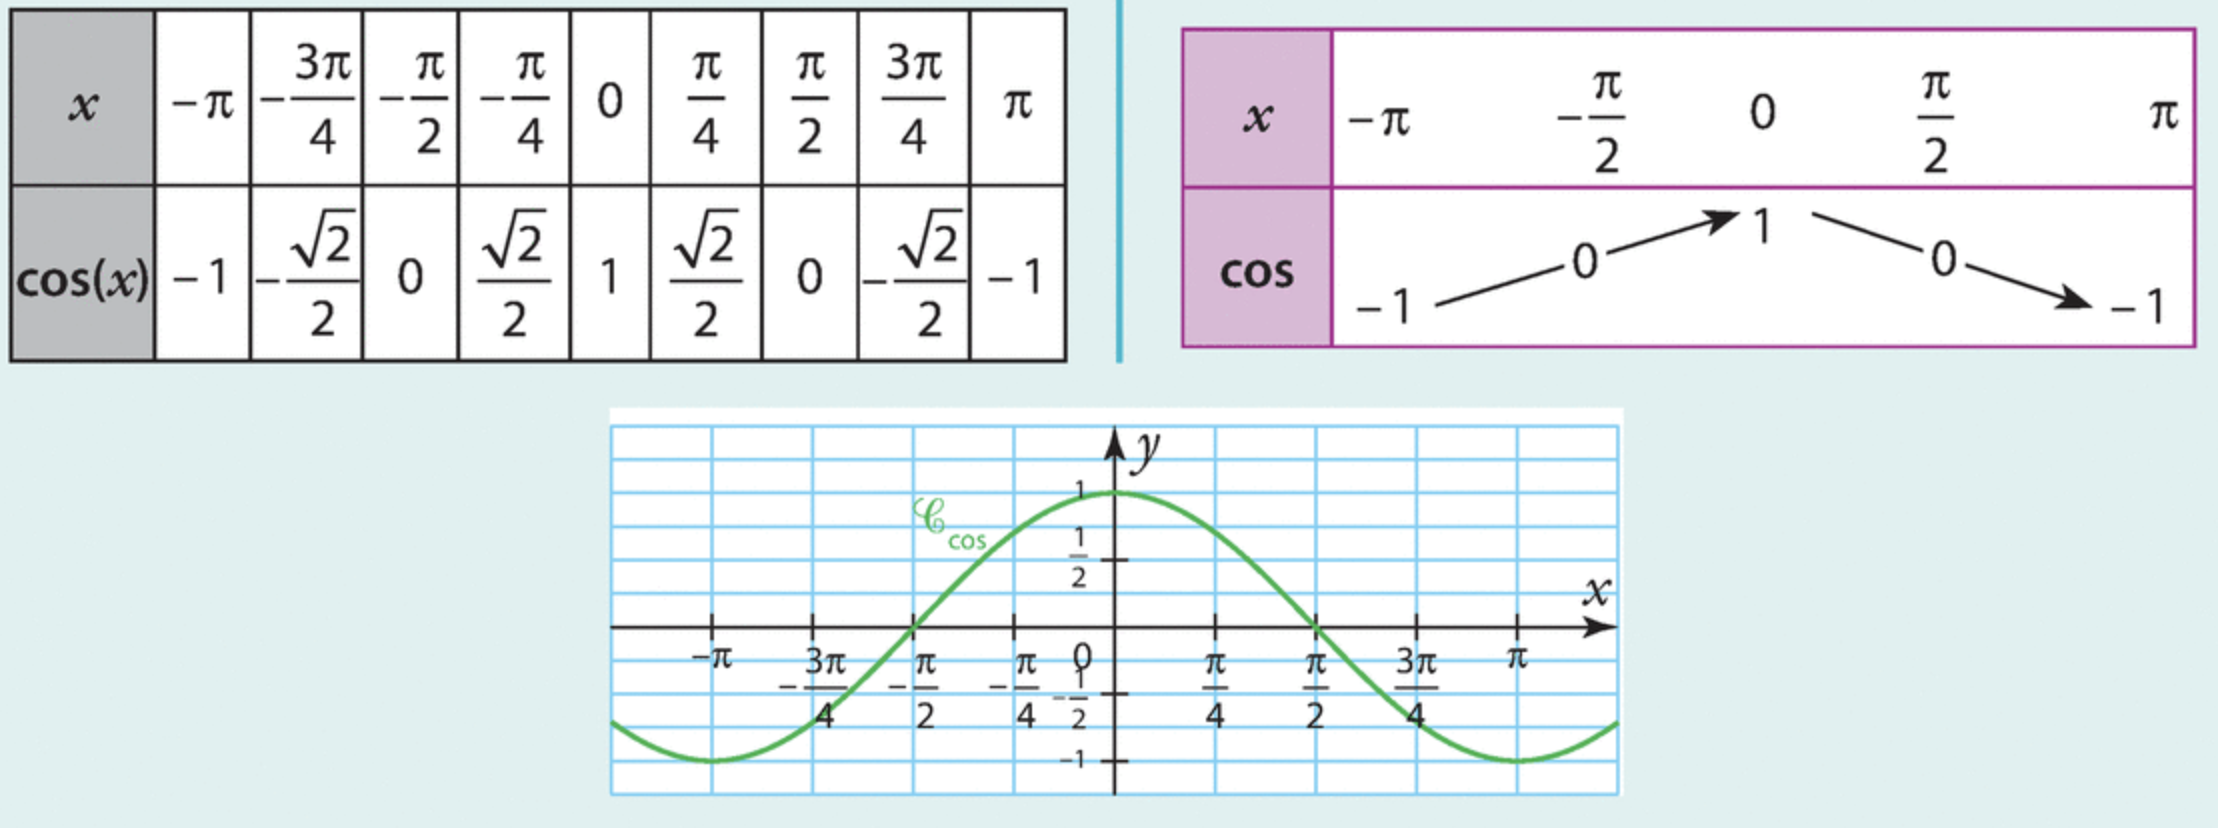
\includegraphics[scale=0.31]{cos_tables.png}
\end{center}
\paragraph*{\underline{Definition}: Sinus function}
Sinus noted $\sin$ defined on $\mathbb{R}$
\begin{center}
    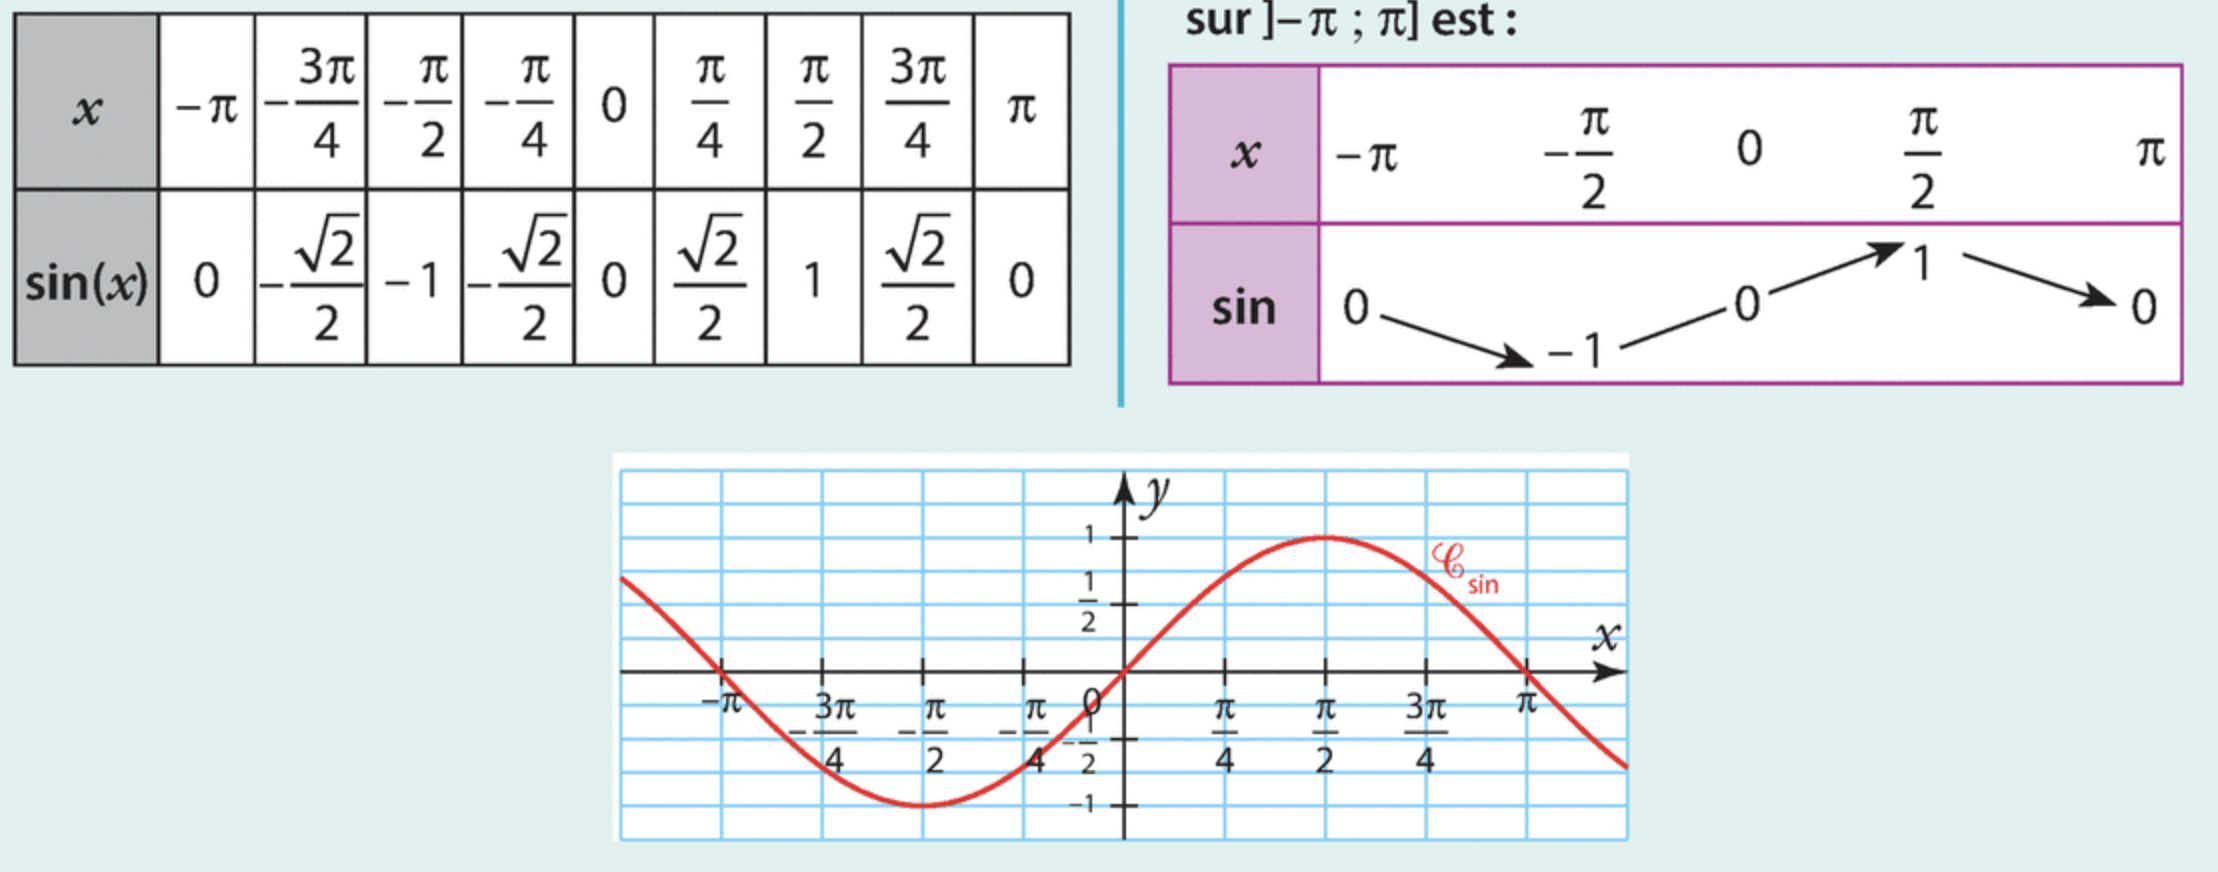
\includegraphics[scale=0.31]{sin_tables.png}
\end{center}
\paragraph{\underline{Property}: Superposition of images-points}
let $x$ a real and $M_x(\cos{x};\sin{x})$. $M_x$ and $M_{x+2\pi}(\cos{x+2\pi};\sin{x+2\pi})$
are confused.

\paragraph*{\underline{Property}: Periodicity}
$\sin$ and $\cos$ are periodic of period $2\pi$
$$\cos{x} = \cos{2\pi+x}$$
$$\sin{x} = \sin{2\pi+x}$$

\paragraph*{\underline{Property}: Parity of sin and cos}
Let $x$ a Real:
\begin{itemize}
    \item sinus is unpair because central symetric with origin
    \item cosinus is pair because axial symetric with ordinate axis
\end{itemize}
\end{document}